 \documentclass[a4paper, 10pt]{article}
\usepackage[banglamainfont=Kalpurush,
           banglattfont=Siyam Rupali]
           {latexbangla}
\usepackage[margin=1in,bottom=2.5in,top=2in]{geometry}
\usepackage{graphicx}
\usepackage{wrapfig}
\usepackage{fancyhdr}
\pagestyle{fancy}
\setlength{\parindent}{0cm}
\setlength{\headheight}{21ex}

\def\bengalinumber#1{\bengalidigits{\number#1}}
\def\bengalinumeral#1{\bengalinumber{\csnamec@#1\endcsname}}
\setmainlanguage[numerals=Bengali,changecounternumbering=false]{bengali}

\linespread{1.2}

\newtheorem{eproblem}{Problem}

\begin{document}

\lhead{ 
\includegraphics[height=20ex]{yearlogo.png} }
\chead{\begin{Large} ডাচ বাংলা ব্যাংক প্রথম আলো গণিত উৎসব ২০২২ \\ জাতীয় গণিত উৎসব \\ আয়োজক: বাংলাদেশ গণিত অলিম্পিয়াড কমিটি \\ \vspace{4pt} \end{Large} }
\rhead{ 
\includegraphics[height=20ex]{MOlogo.png} }

\lfoot{১১ মার্চ ২০২২}
\rfoot{সেন্ট যোসেফ হায়ার সেকেন্ডারি স্কুল, আসাদ এভিনিউ, ঢাকা}

\begin{tabular}{lcr}
ক্যাটাগরি: সেকেন্ডারি (৯ম - ১০ম শ্রেণী)  & \hspace{34ex} & সময়: ৪ ঘণ্টা \\
Category: Secondary (9th grade - 10th grade) & & Time: 4 hours \\
\end{tabular}

\vspace{2ex}

\textbf{সমস্যাগুলো কাঠিন্য অনুসারে সাজানোর চেষ্টা করা হয়েছে।প্রতিটি সমস্যার পূর্ণমান তার পাশে দেওয়া আছে।প্রশ্নের নম্বর ব্যতীত প্রতিটি সংখ্যা ইংরেজিতে লেখা। সমস্যার সমাধান মূল উত্তরপত্রে লিখতে হবে। রাফ করার জন্য মূল উত্তরপত্রের পিছনের অংশ ব্যবহার করা যাবে। বাড়তি কাগজ নিলে সেখানে নাম ও রেজিস্ট্রেশন নম্বর লেখা বাঞ্ছনীয়।}

\begin{problem}
প্রমাণ কর, $a,b,c$ ধনাত্মক বাস্তব সংখ্যা হলে,
$$\dfrac{a}{bc}+\dfrac{b}{ca}+\dfrac{c}{ab}\ge \dfrac{2}{a}+\dfrac{2}{b}-\dfrac{2}{c}$$
\end{problem}

\begin{eproblem}
Prove that, if $a,b,c$ are positive real numbers,
$$\dfrac{a}{bc}+\dfrac{b}{ca}+\dfrac{c}{ab}\ge \dfrac{2}{a}+\dfrac{2}{b}-\dfrac{2}{c}$$
\end{eproblem}

\begin{problem}
এমন সব মৌলিক সংখ্যা বের কর যাদের বর্গকে দু'টি ধনাত্মক পুর্ণসংখ্যার ঘনের যোগফল হিসেবে লেখা যাবে।
\end{problem}

\begin{eproblem}
Find all prime numbers such that the square of the prime number can be written as the sum of cubes of two positive integers.
\end{eproblem}

\begin{problem}
$\alpha$ এবং $\omega$ দু'টি বৃত্ত যাতে $\omega$, $\alpha$ এর কেন্দ্র দিয়ে যায়। বৃত্ত দুইটি $A$ এবং $B$ বিন্দুতে ছেদ করে। $P$, $\omega$ এর পরিধির ওপরে কোন বিন্দু। $PA$ এবং $PB$, $\alpha$ কে আবার যথাক্রমে $E$ এবং $F$ বিন্দুতে ছেদ করে। প্রমাণ কর যে, $AB=EF$.
\end{problem}

\begin{eproblem}
Let $\alpha$ and $\omega$ be $2$ circles such that $\omega$ goes through the center of $\alpha$. $\omega$ intersects $\alpha$ at  $A$ and $B$. Let $P$ be any point on the circumference $\omega$. The lines $PA$ and $PB$ intersects $\alpha$ again at $E$ and $F$ respectively. Prove that $AB=EF$.
\end{eproblem}

\begin{center}
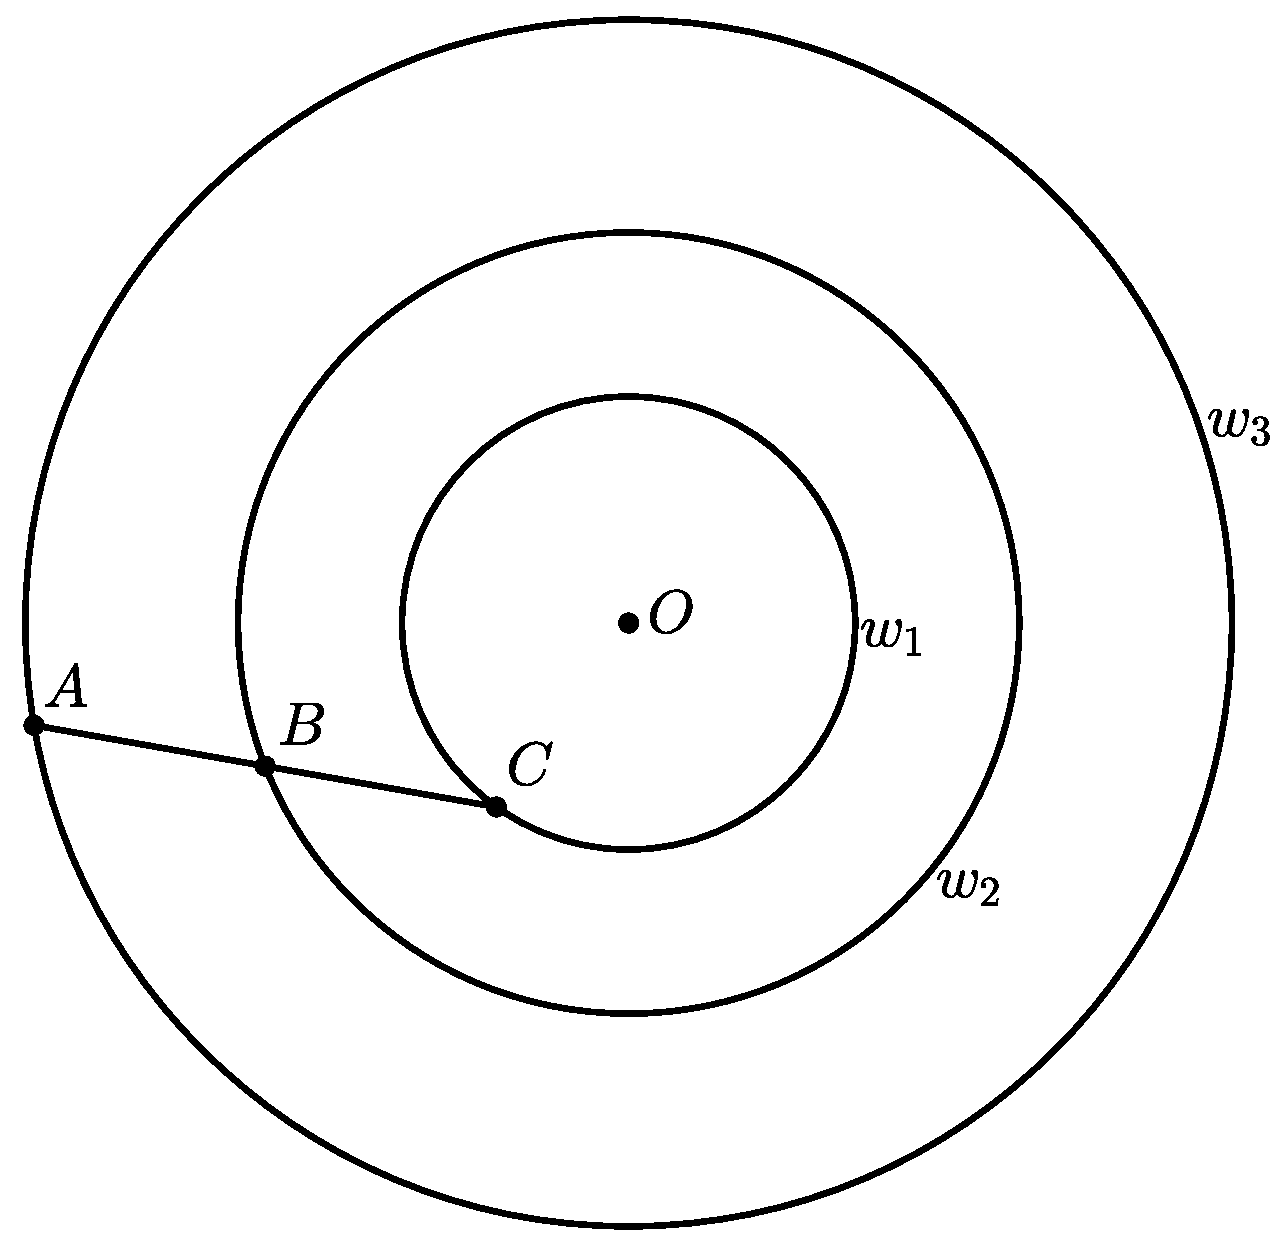
\includegraphics[width=0.25\textwidth]{geo}
\end{center}


\end{document}